%%
%% Created in 2018 by Martin Slapak
%%
%% Based on file for NRP report LaTeX class by Vit Zyka (2008)
%%
%% Compilation:
%% >pdflatex report
%% >bibtex report
%% >pdflatex report
%% >pdflatex report

\documentclass[czech]{mvi-report}

\usepackage[utf8]{inputenc}
\usepackage{amsmath}
\usepackage{colortbl}
\usepackage{listings}

\usepackage{graphicx}
\graphicspath{ {./img/} }

\title{DÚ č.1 - Entropie a kódování}

\author{Marek Nevole, Jan Novotný}
\affiliation{ČVUT - FIT}
\email{\{nevolmar, novot103\}@fit.cvut.cz}

\def\file#1{{\tt#1}}

\begin{document}

\maketitle

%%%%%%%%%%%%%%%%%%%%%%%%%%%%%%%%%%%%%%%%%%%%%%%%%%%%%%%%%%%%%%%%%%%%%%%%%%%%%%%%
\section{Úvod}
První úkol z předmětu vybrané statistické metody byl na téma entropie a kódování. Za reprezentanta byl zvolen Marek Nevole.

\begin{align*}
  K &= 28\\
  L &= 6\\
  X &= ((23KL)\text{ mod }20) + 1\\
  X &= 5\\
  Y &= ((X + ((5K + 7L)\text{ mod }19))\text{ mod }20) + 1\\
  Y &= 17
\end{align*}

Výsledkem těchto rovnic jsou názvy vybraných datových souborů. V našem případě budeme pracovat se soubory 005.txt a 017.txt.

Úkol byl vypracován pomocí programovacího jazyku Python\footnote{python.org} v prostředí Jupyter Notebook\footnote{jupyter.org} s volně dostupnou knihovnou SciPy\footnote{scipy.org} a Matplotlib\footnote{matplotlib.org}.

\section{Úloha č.1}
\textit{Z obou datových souborů načtěte texty k analýze. Pro každý text zvlášť odhadněte pravděpodobnosti znaků (symbolů včetně mezery), které se v textech vyskytují. Výsledné pravděpodobnosti graficky znázorněte.}\\

Pokud mluvíme o prvním textu, myslíme text ze souboru \textbf{005.txt} a náhodnou veličinu znaků značíme $ X_1 $, obdobně druhým textem máme na mysli text z \textbf{017.txt} a náhodnou veličinu znaků značíme $ X_2 $. Část prvního textu, určená k analýze, obsahuje 5410 znaků vč. mezer. Druhý text obsahuje více znaků, konkrétně 6709. Částí k analýze je myšlen text bez prvního řádku.

Na obrázku \ref{fig:aprob} můžeme pozorovat překrývající se absolutní četnosti znaků obou textů. Rozdělění znaků je velice obdobné až na určitou odchylku určenou absolutním rozdílem počtu znaků textů. Nepřekvapivě je nejčastějším znakem mezera. Nejčastěji použitým znakem z abecedy je \textit{e}.

\begin{figure}[ht!]
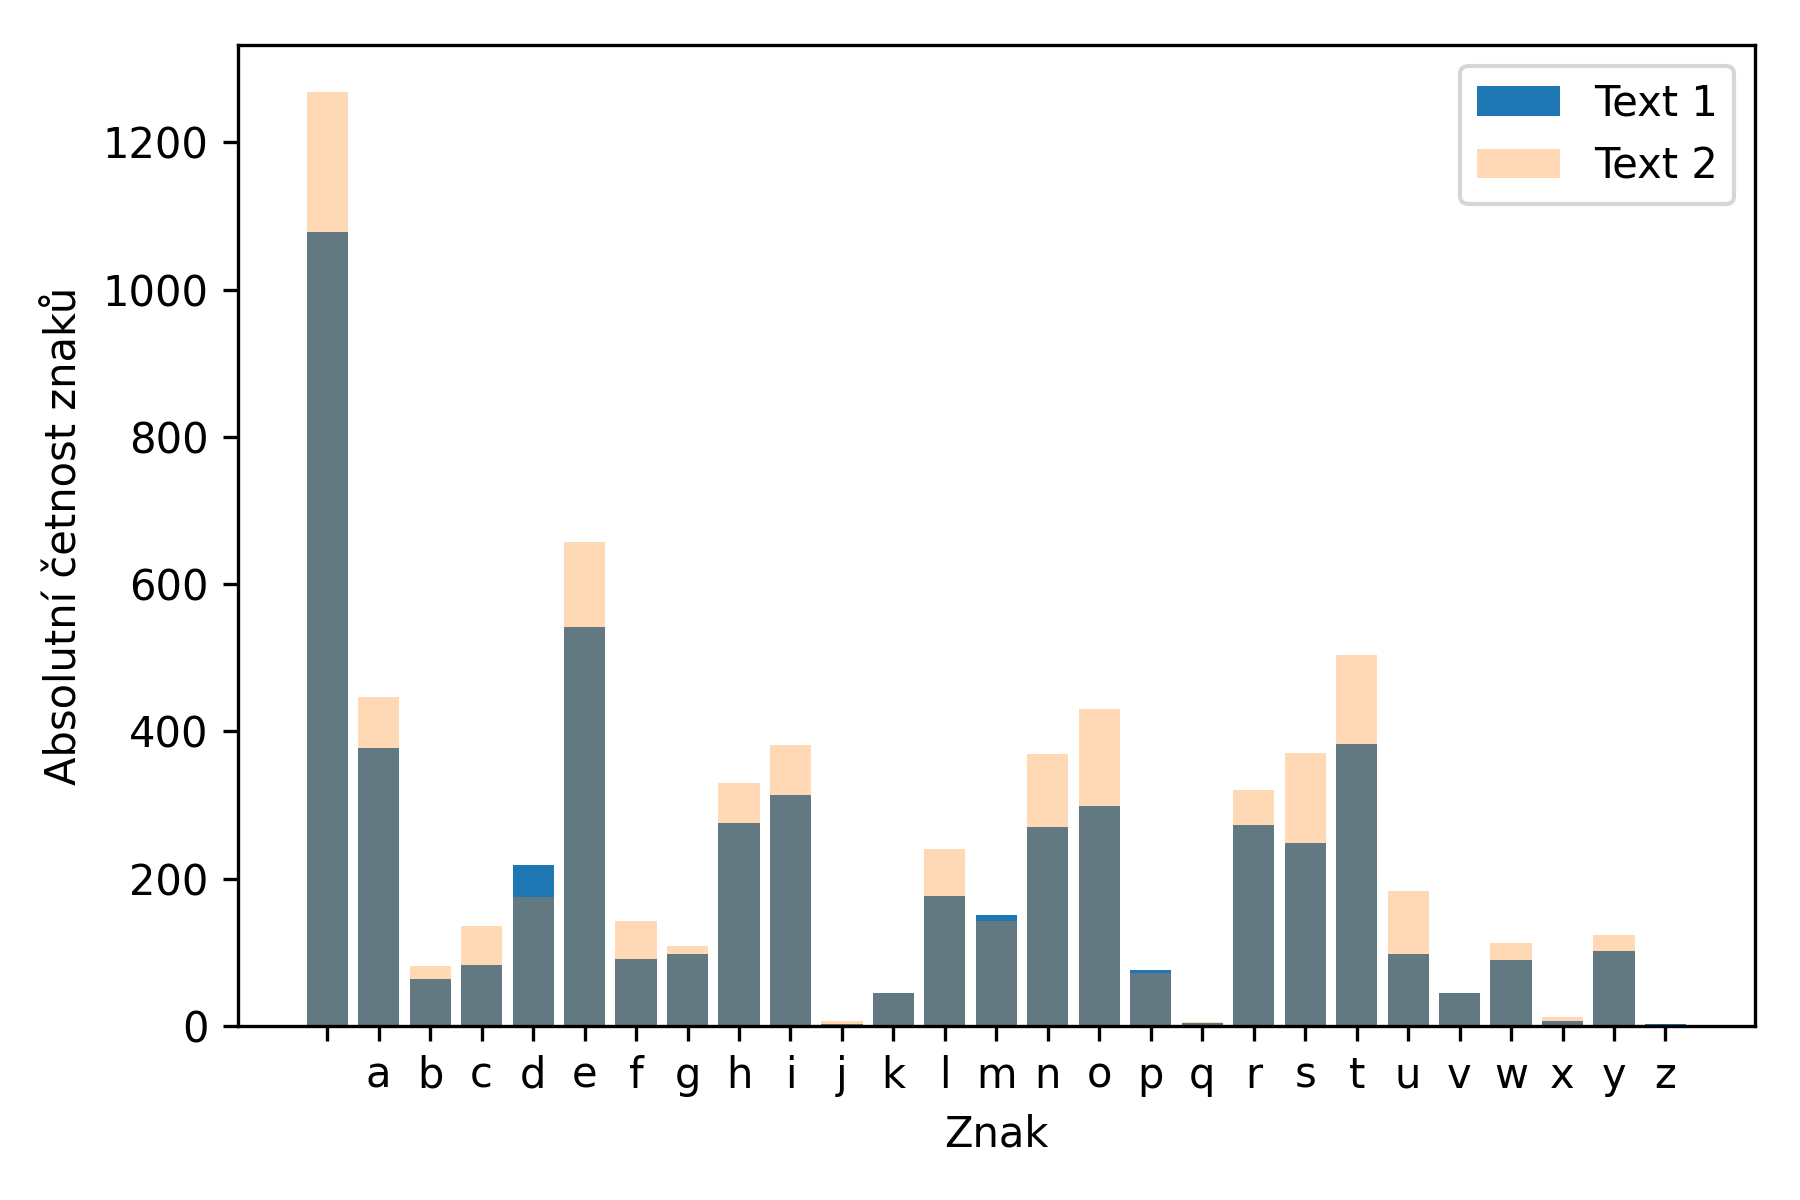
\includegraphics[width=\columnwidth]{aprob1.png}
\caption{Absolutní četnost znaků ve zkoumaných textech.}
\label{fig:aprob}
\end{figure}

Překrývající se relativní četnosti znaků v textech je na obrázku \ref{fig:rprob}. Odchylka je zde ještě menší, tedy rozdělení znaků v těchto textech je téměř stejné. Relativní četnosti budem dále používat jako odhadované pravděpodobnosti výskytu znaků.

\begin{figure}[ht!]
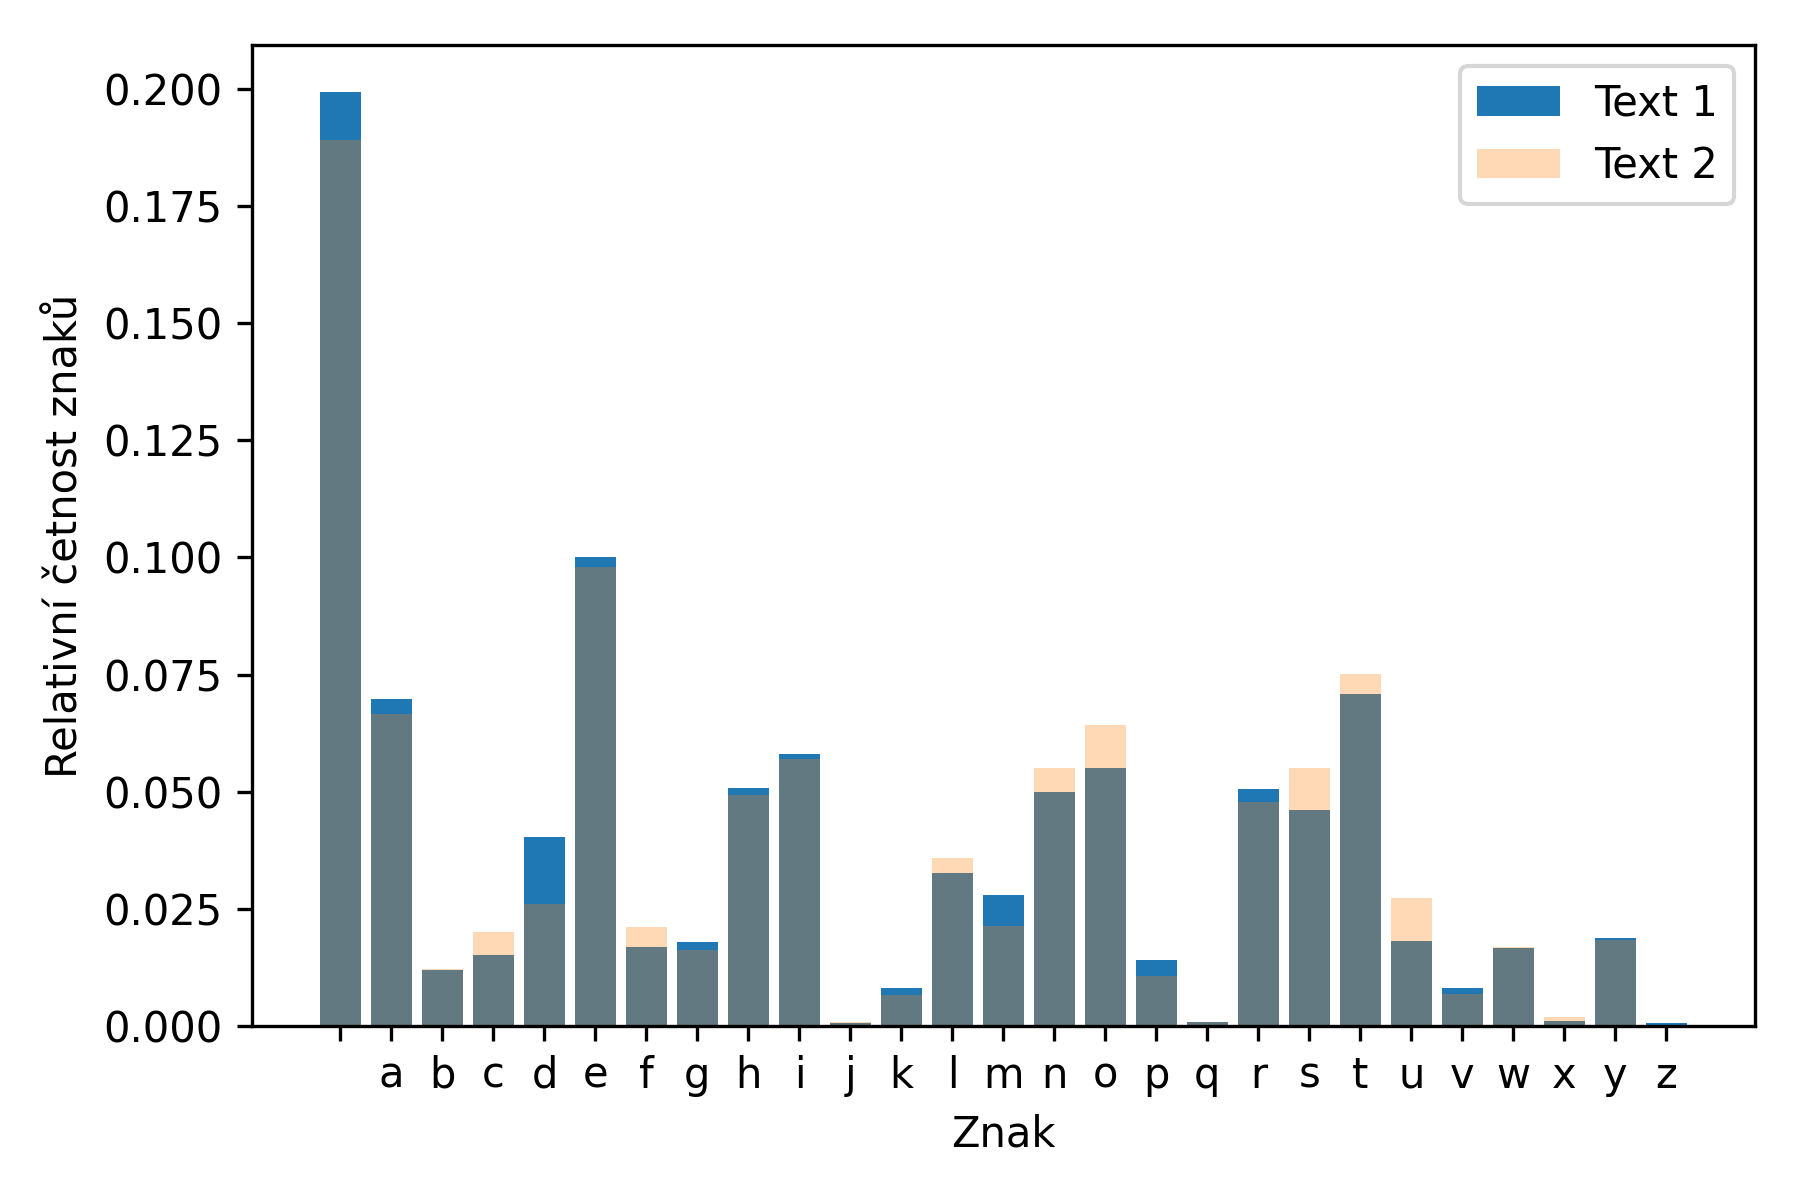
\includegraphics[width=\columnwidth]{rprob1.png}
\caption{Relativní četnost znaků ve zkoumaných textech.}
\label{fig:rprob}
\end{figure}

\section{Úloha č.2}
\textit{Pro každý text zvlášť spočtěte entropii odhadnutého rozdělení znaků.}\\

Pro následující úlohy, ve kterých budeme sestavovat optimální binární instatní kód, budeme počítat entropii s logaritmem o základu 2 značenou $H_2$. Jednotkou entropie bude bit. Entropii pro každý text zvlášť jsme vypočítali pomocí funkce \textit{scipy.stats.entropy()} z relativních četností znaků.
\begin{align*}
  H_2(X_1) &= 4.063 \text{ bitu}\\
  H_2(X_2) &= 4.078 \text{ bitu}
\end{align*}

Hodnoty entropií splňují větu o maximalizaci entropie, která říka, že $H(X) \leq \log(|X|)$, což obě entropie splňují, jelikož pro oba texty je $\log(|X_1|) = \log(|X_2|) = 4.755$. Entropie jsou velice podobné, což odpovídá velice podobným relativním četnostem znaků.

\noindent\rule{\columnwidth}{1pt}
\begin{lstlisting}[language=Python]
from scipy.stats import entropy

e1 = entropy(p1, base = 2)
\end{lstlisting}
\noindent\rule{\columnwidth}{1pt}


\section{Úloha č.3}
\textit{Nalezněte optimální binární instantní kód $C$ pro kódování znaků \textbf{prvního} z textů.}\\

Cílem úlohy bylo nalézt optimální binární instantní kód pro kódování znaků prvního z textů. Tento kód získáme pomocí algoritmu Huffmanova kódování, který zaručí požadované vlastnosti.
Získaná kódová slova pro všechny znaky lze pozorovat v tabulce \ref{tab:codebook}.

\begin{table}
  \caption{Kódovací tabulka kódu $C_1$ vytvořena z četností znaků z $X_1$}
  \centering
  \begin{tabular}{|ccc|ccc|}
  \hline
  \rowcolor[rgb]{0.722,0.722,0.722} $x$ & $C(x)$        & $l$  & $x$ & $C(x)$        & $l$   \\
  \hline
  \rowcolor[rgb]{0.82,0.82,0.82} ' '  & 00          & 2  & n & 0100        & 4   \\
  \rowcolor[rgb]{0.941,0.941,0.941} a & 1011        & 4  & o & 0111        & 4   \\
  \rowcolor[rgb]{0.722,0.722,0.722} b & 1110010     & 7  & p & 1110011     & 7   \\
  \rowcolor[rgb]{0.82,0.82,0.82} c    & 100110      & 6  & q & 1110001010  & 10  \\
  \rowcolor[rgb]{0.941,0.941,0.941} d & 11011       & 5  & r & 0101        & 4   \\
  \rowcolor[rgb]{0.722,0.722,0.722} e & 1111        & 4  & s & 11101       & 5   \\
  \rowcolor[rgb]{0.82,0.82,0.82} f    & 101010      & 6  & t & 1100        & 4   \\
  \rowcolor[rgb]{0.941,0.941,0.941} g & 101011      & 6  & u & 110100      & 6   \\
  \rowcolor[rgb]{0.722,0.722,0.722} h & 0110        & 4  & v & 11100011    & 8   \\
  \rowcolor[rgb]{0.82,0.82,0.82} i    & 1000        & 4  & w & 100111      & 6   \\
  \rowcolor[rgb]{0.941,0.941,0.941} j & 11100010111 & 11 & x & 111000100   & 9   \\
  \rowcolor[rgb]{0.722,0.722,0.722} k & 1110000     & 7  & y & 110101      & 6   \\
  \rowcolor[rgb]{0.82,0.82,0.82} l    & 10100       & 5  & z & 11100010110 & 11  \\
  \rowcolor[rgb]{0.941,0.941,0.941} m & 10010       & 5  &   &             &     \\
  \hline
  \end{tabular}
  \label{tab:codebook}
  \end{table}

Algoritmus pro získání Huffmanova kódu jsme v rámci procvičení implementovali sami. Kvůli délce kódu zde popíšeme algoritmus pouze slovně.

\noindent\rule{\columnwidth}{1pt}
\begin{enumerate}
  \item Sestavíme minimovou haldu ze dvojic skládájících se ze znaku a jeho četnosti(nezáleží zda je relativní nebo absolutní). Řadíme podle četnosti.
  \item Sestavíme Huffmanův strom, tak že dokud má halda více než 1 dvojici, tak odebereme nejmenší 2 dvojice, pro které vytvoříme novou dvojici, které přiřadíme menší dvojici jako levého potomka a zbylou dvojici jako pravého potomka, četnost této dvojice nastavíme na součet 2 odebraných dvojic. Novou dvojici vložíme do haldy. Poslední prvek, který v haldě zůstane je kořen Huffmanova stromu.
  \item Od kořene rekurzivně procházíme strom směrem k listům, hranám, které vedou k levým potomkům přiřazujeme znak 1, jinak 0. Kódové slovo pro znak poté získáme poskládáním znaků hran po cestě od kořene k listu s uvedeným znakem.
\end{enumerate}
\noindent\rule{\columnwidth}{1pt}


\section{Úloha č.4}
\textit{Pro každý text zvlášť spočtěte střední délku kódu $C$ a porovnejte ji s entropií rozdělení znaků. Je kód $C$ optimální i pro \textbf{druhý} text?}\\

Střední délky kódu pro oba texty jsme spočetli podle uvedeného vzorce z přednášek, kde za $p(x)$ jsme vzali získané relativní četnosti znaků a vynásobili je délkami kódových slov z $C_1$.

\begin{align*}
  H_2(X_1) &= 4.063 \text{ bitu}\\
  L_1(C_1) &= 4.107\\
  H_2(X_2) &= 4.078 \text{ bitu}\\
  L_2(C_1) &= 4.136
\end{align*}
Spočtené střední délky kódů, jak bylo pro Huffmanův kód předpokládáno, splňují rovnost $L(C) \geq H_2(X)$, a také nejsou vzdálené od entropie o více než 1.
Abychom zjistili, zda je kód $C_1$ optimální i pro rozdělení znaků ve druhém textu, tak jsme sestavili kód $C_2$.
\begin{equation*}
  L_2(C_2) = 4.121
\end{equation*}

Střední délka kódu $C_2$ je pro druhý text menší než $C_1$, tedy $C_1$ není optimálním kódem pro druhý text.

\end{document}
